\documentclass{llncs}
\usepackage{parskip, graphicx, minted}
\usepackage[bottom=1.5cm, right=1.5cm, left=1.5cm, top=1.5cm]{geometry}

\begin{document}

\title{Database Design}
\subtitle{D Simulator}
\author{Issac Yang, Yuxiang Lin, Shanruo Xu}
\institute{Duke Kunshan University}

\maketitle

\section{ER Diagram}

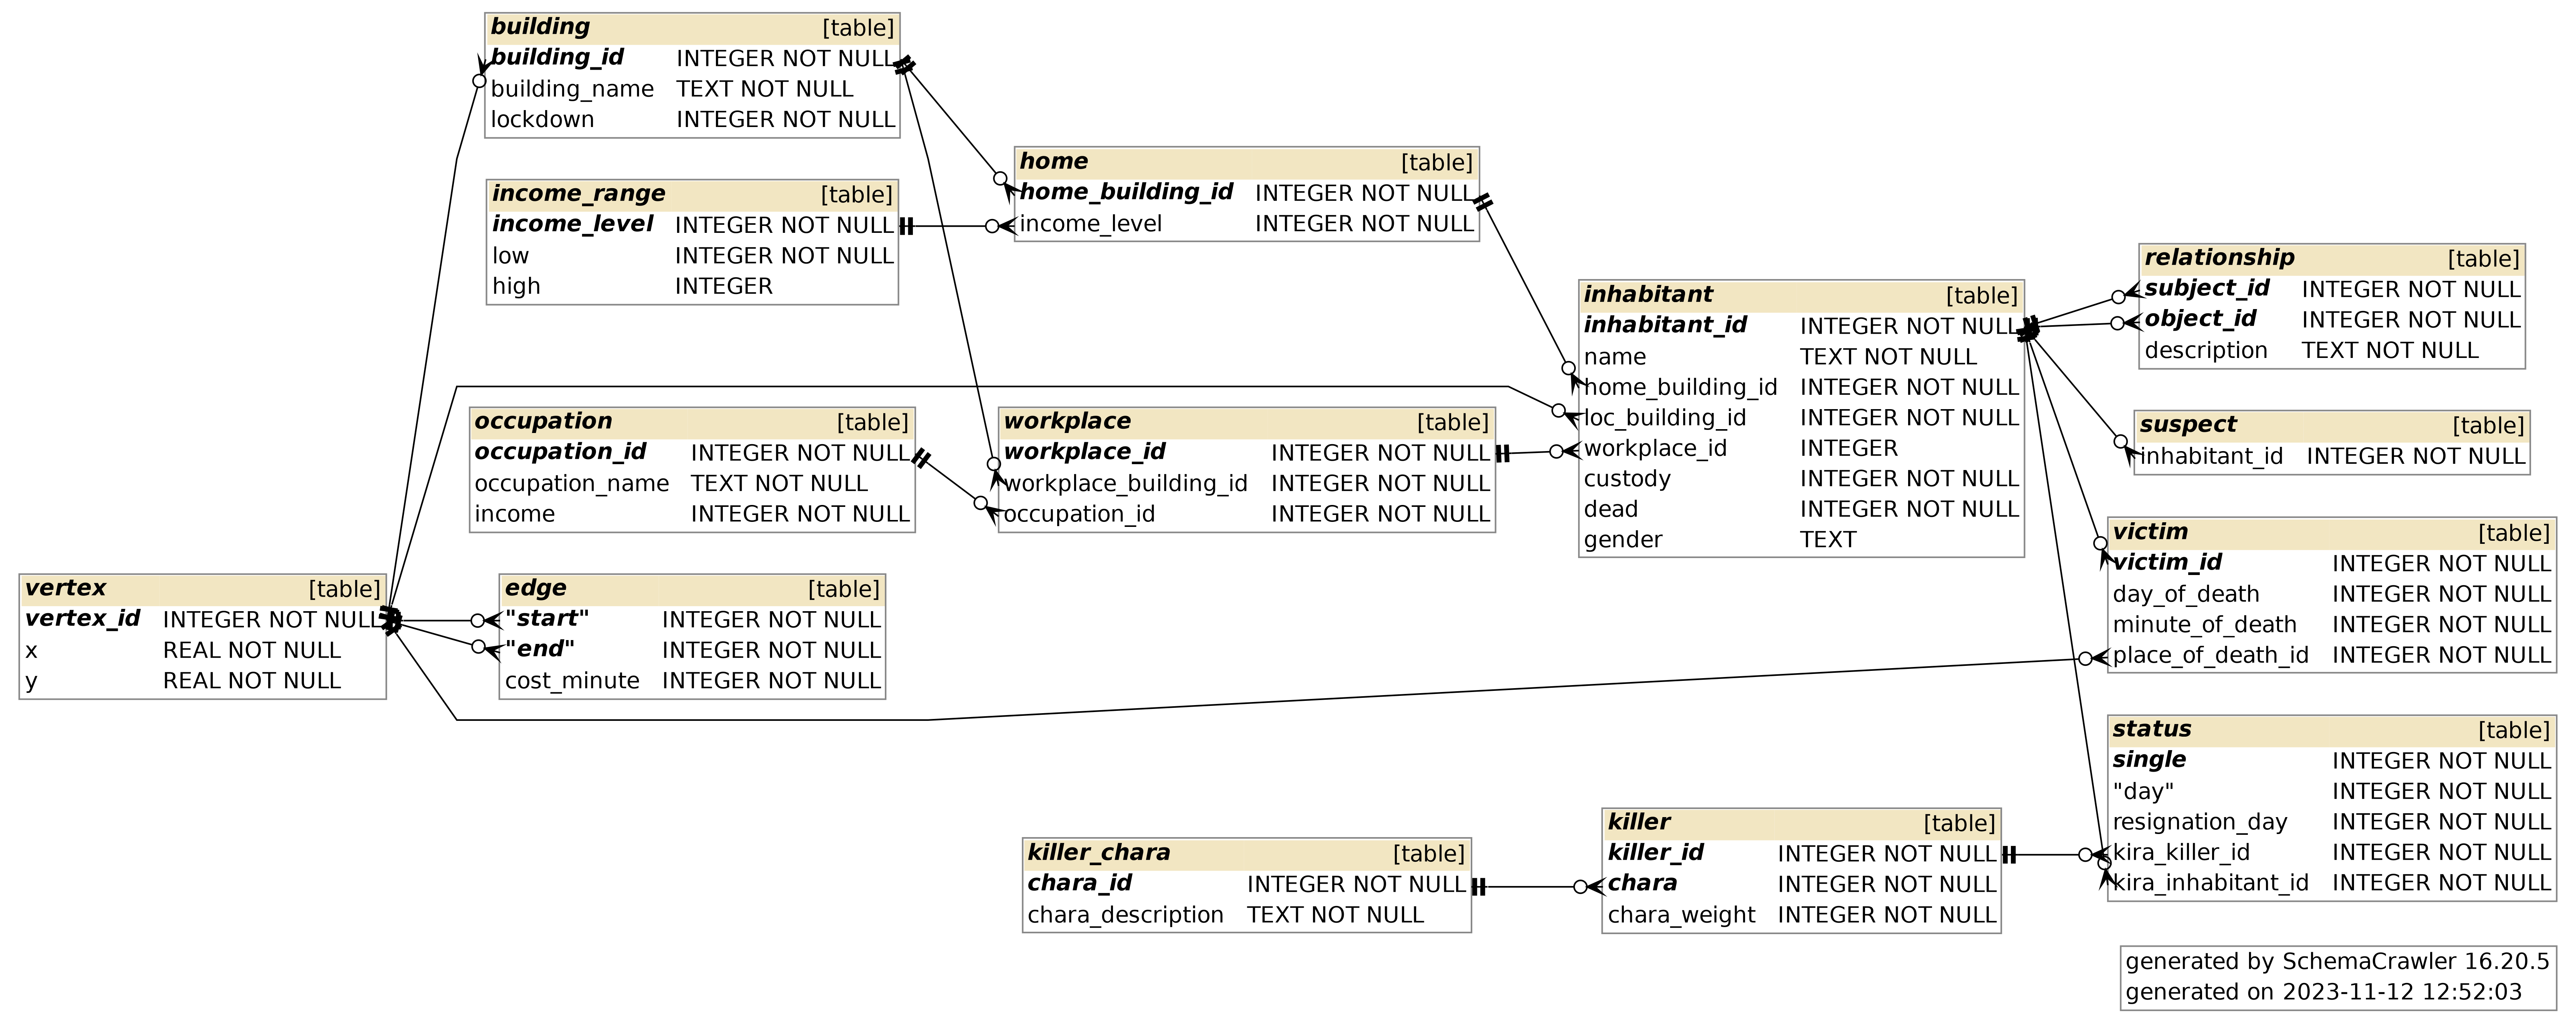
\includegraphics[width=\textwidth]{diagram.png}

\section{Database Schema}

This database is to be implemented in SQLite. SQLite is dynamic-typed with only these five storage classes: \textbf{NULL, INTEGER, REAL, TEXT, BLOB}. Therefore, all string data would be simply stored as \textbf{TEXT}. For boolean type, it is stored as an \textbf{INTEGER} constrained to be either 0 or 1 to represent \textbf{TRUE} or \textbf{FALSE}. All SQLite tables have a \textbf{ROWID} column by default unless \textbf{WITHOUT ROWID} is specified. The specification of a column as \textbf{INTEGER PRIMARY KEY} usually results in an alias to \textbf{ROWID}, which is a 64-bit integer that uniquely identifies each row.

\inputminted[firstline=1,lastline=6]{sql}{DDL.sql}
Stores information about vertices representing locations.

\inputminted[firstline=8,lastline=15]{sql}{DDL.sql}
Describes edges connecting vertices, including the cost in minutes to traverse the edge.

\inputminted[firstline=17,lastline=23]{sql}{DDL.sql}
Represents information about homes, linking them to specific income levels.

\inputminted[firstline=25,lastline=31]{sql}{DDL.sql}
Stores income range levels along with corresponding low and high values.

\inputminted[firstline=33,lastline=39]{sql}{DDL.sql}
Represents information about homes, linking them to specific income levels.

\inputminted[firstline=41,lastline=46]{sql}{DDL.sql}
Contain information about occupation as well as their income level.

\inputminted[firstline=48,lastline=56]{sql}{DDL.sql}
Link occupation accordingly to their specific workplace.

\inputminted[firstline=58,lastline=71]{sql}{DDL.sql}
Include information about the inhabitants, including homes workplace, dead status, gender, etc.

\inputminted[firstline=73,lastline=80]{sql}{DDL.sql}
Record and describe the relationship between inhabitants.

\inputminted[firstline=82,lastline=90]{sql}{DDL.sql}
Contains information about victims, including the time and place of death.

\inputminted[firstline=92,lastline=98]{sql}{DDL.sql}
Stores information about killers and their characteristics.

\inputminted[firstline=100,lastline=106]{sql}{DDL.sql}
Store the killer characters that will influence the potential victims, as well as the detailed description about how exactly it will influence this choice.

\inputminted[firstline=106,lastline=109]{sql}{DDL.sql}
Put the suspect the player chose to the list

\inputminted[firstline=111,lastline=120]{sql}{DDL.sql}
Stores status information, including relationship status and details related to a specific killer. This is forced to be a single row as these all the "global" attributes. By forcing the special primary key \textbf{single} to always be 0 and disable \textbf{ROWID}, such a single row constraint is enforced.

\end{document}
